
\section{Dataset}\label{sec:dataset}

We use InsectSet66~\cite{insectset66zenodo}, a public dataset of field recordings from 66 insect species belonging to the orders Orthoptera (grasshoppers, crickets) and Cicadidae (cicadas).
The dataset contains 2,887 mono WAV files with official train, validation, and test splits.
Table~\ref{tab:splits} shows the number of recordings per subset.
Species representation is imbalanced, ranging from 10 to 160 recordings per species (median 35).
This motivates reporting macro-averaged F1 alongside accuracy.

\begin{table}[!t]
\caption{InsectSet66 recording counts by subset.}
\label{tab:splits}
\centering
\begin{tabular}{lrr}
\toprule
Subset & Recordings & Chunks \\
\midrule
Train      & 1{,}752 & 41{,}312 \\
Validation & 579     & 12{,}587 \\
Test       & 556     & 10{,}391 \\
\midrule
Total      & 2{,}887 & 64{,}290 \\
\bottomrule
\end{tabular}
\end{table}

\section{Methods}\label{sec:methods}

\subsection{Segmentation}

Each recording is split into 5-second chunks with 3.75~s overlap (1.25~s advance step).
Short recordings are loop-padded to reach 5~s.
The final partial segment is kept if it exceeds 1.25~s.
This yields 64,290 chunks across all subsets, as shown in Table~\ref{tab:splits}.
All waveforms are resampled to 44.1~kHz mono.
The official file-level splits are preserved so that chunks from the same recording always belong to the same subset.

\subsection{Feature extraction}

\subsubsection{Log-mel spectrogram (CNN baseline)}
Each 5-second chunk is transformed into a log-mel spectrogram.
A short-time Fourier transform (STFT) is applied with $n_{\text{FFT}}=1000$, hop length 147, and window length 294.
The power spectrum is mapped to 64 mel-frequency bands and converted to a decibel scale using \texttt{AmplitudeToDB} with \texttt{top\_db}=80.
The resulting $64 \times 1501$ image is the input to the CNN.
Figure~\ref{fig:logmel} illustrates an example log-mel spectrogram.

\begin{figure}[!t]
    \centering
    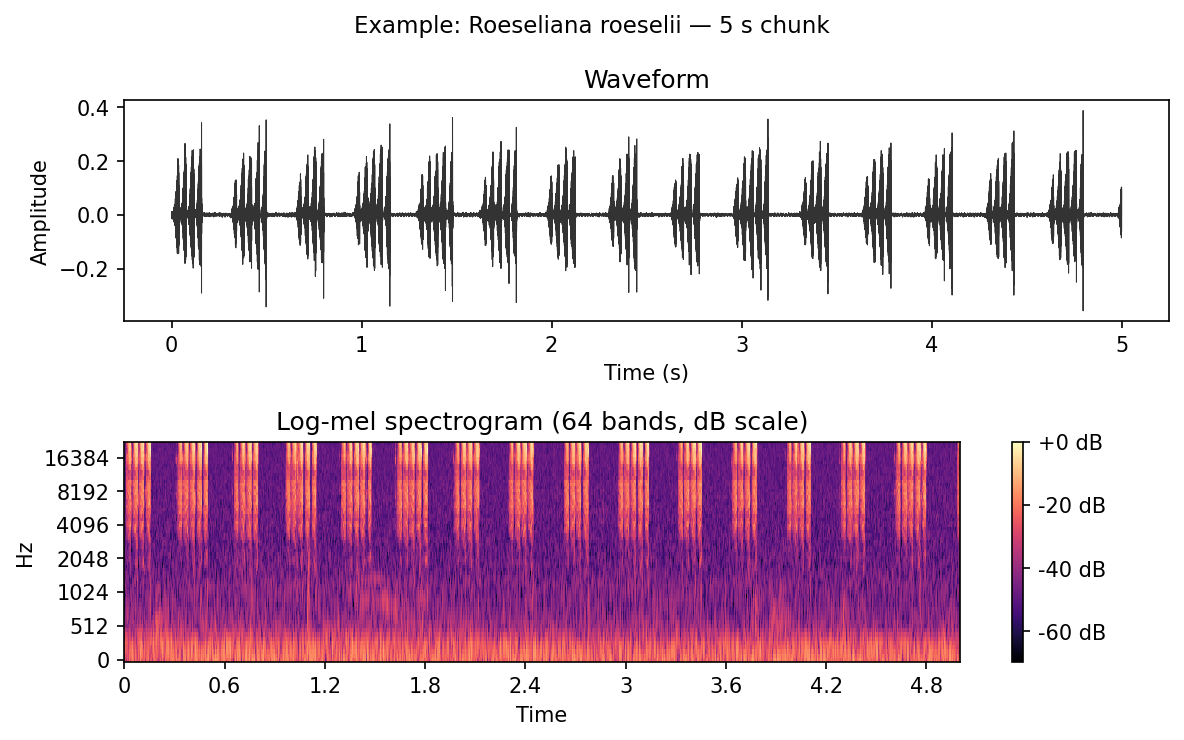
\includegraphics[width=\columnwidth]{images/logmel_baseline_example.png}
    \caption{Example log-mel spectrogram (64 mel bands, log-power in dB). Time is on the horizontal axis and mel frequency on the vertical axis.}
    \label{fig:logmel}
\end{figure}

\subsubsection{MFCC statistical features (classical pipeline)}
We extract 20 Mel-frequency cepstral coefficients (MFCCs) per frame using $n_{\text{FFT}}=2048$ and hop length 512~\cite{mcfee2015librosa}.
First- and second-order delta coefficients capture temporal dynamics.
For each chunk, we compute the mean and standard deviation of each coefficient across all frames, yielding a fixed 120-dimensional feature vector:
20 coefficients $\times$ 3 groups (MFCC, $\Delta$, $\Delta^2$) $\times$ 2 statistics (mean, std).
Feature vectors are standardized to zero mean and unit variance before SVM training.

\subsection{Models}

\subsubsection{Log-mel CNN (baseline replication)}
We replicate the 5-layer convolutional classifier from Faiss et al.~\cite{faiss2023github}.
The network applies five Conv2d blocks (8, 16, 32, 64, 128 channels) with BatchNorm and ReLU activations, followed by global average pooling and a linear output layer for 66 classes.
Training uses Adam with OneCycleLR scheduling and early stopping on validation loss (patience 8).
Data augmentation (colored noise and impulse responses) is disabled in our replication due to missing assets.
Figure~\ref{fig:cnn_arch} illustrates the full network architecture.

\begin{figure}[!t]
    \centering
    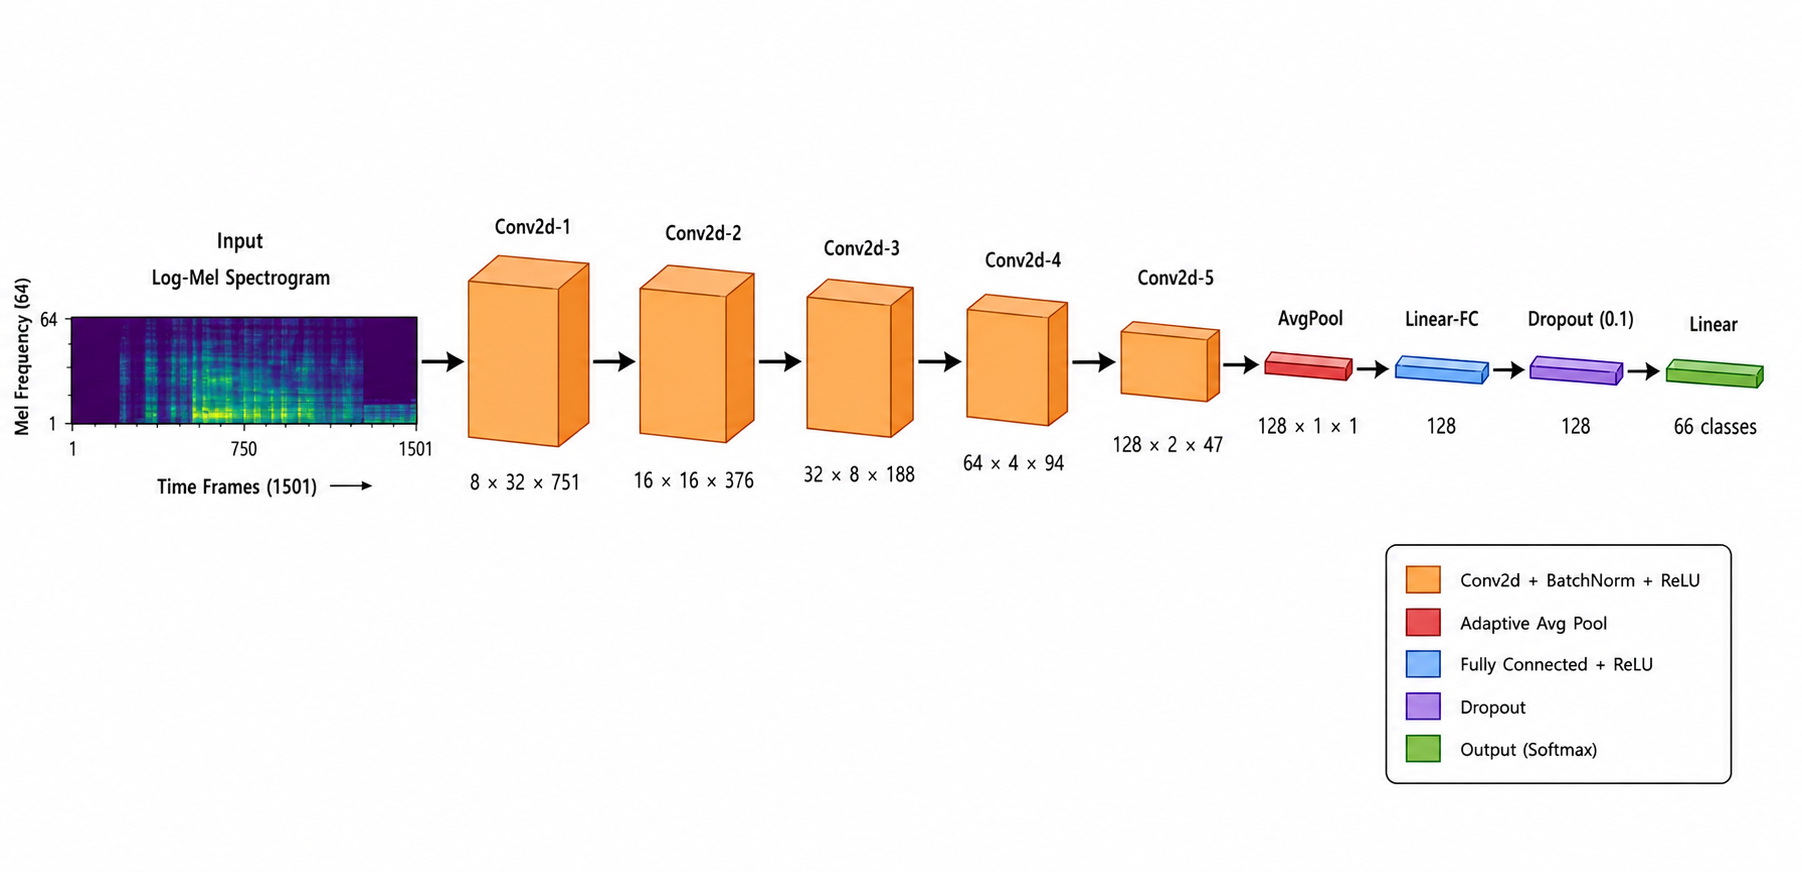
\includegraphics[width=\columnwidth]{images/CNN_architecture.png}
    \caption{Proposed CNN architecture for log-mel spectrogram features. The input $1{\times}64{\times}1501$ tensor passes through five Conv2d blocks (each followed by BatchNorm and ReLU), with stride~2 for progressive downsampling. Global average pooling collapses the spatial dimensions to a 128-d vector, which is passed through dropout and a linear layer to produce 66 class logits.}
    \label{fig:cnn_arch}
\end{figure}

\subsubsection{Support Vector Machine}
We train an SVM with an RBF kernel, $C=10$, and \texttt{class\_weight=balanced} on the scaled 120-dimensional MFCC vectors.
The balanced class weighting compensates for species imbalance.

\subsubsection{Random Forest}
We train a Random Forest with 200 trees and \texttt{class\_weight=balanced} on the unscaled MFCC vectors.
Feature importance scores (Gini impurity) are used for interpretability analysis.

\subsection{Evaluation metrics}

We report \textbf{accuracy} and \textbf{macro-averaged F1} on the held-out test set.
Macro-F1 averages F1 equally across all 66 classes and is more informative than accuracy under class imbalance.
Confusion matrices are visualized as heatmaps.
